\section{Background on Wearable Device Authentication}
\label{sec:background}

\begin{figure*}[t]
\begin{center}
\begin{tabular}{ccc}
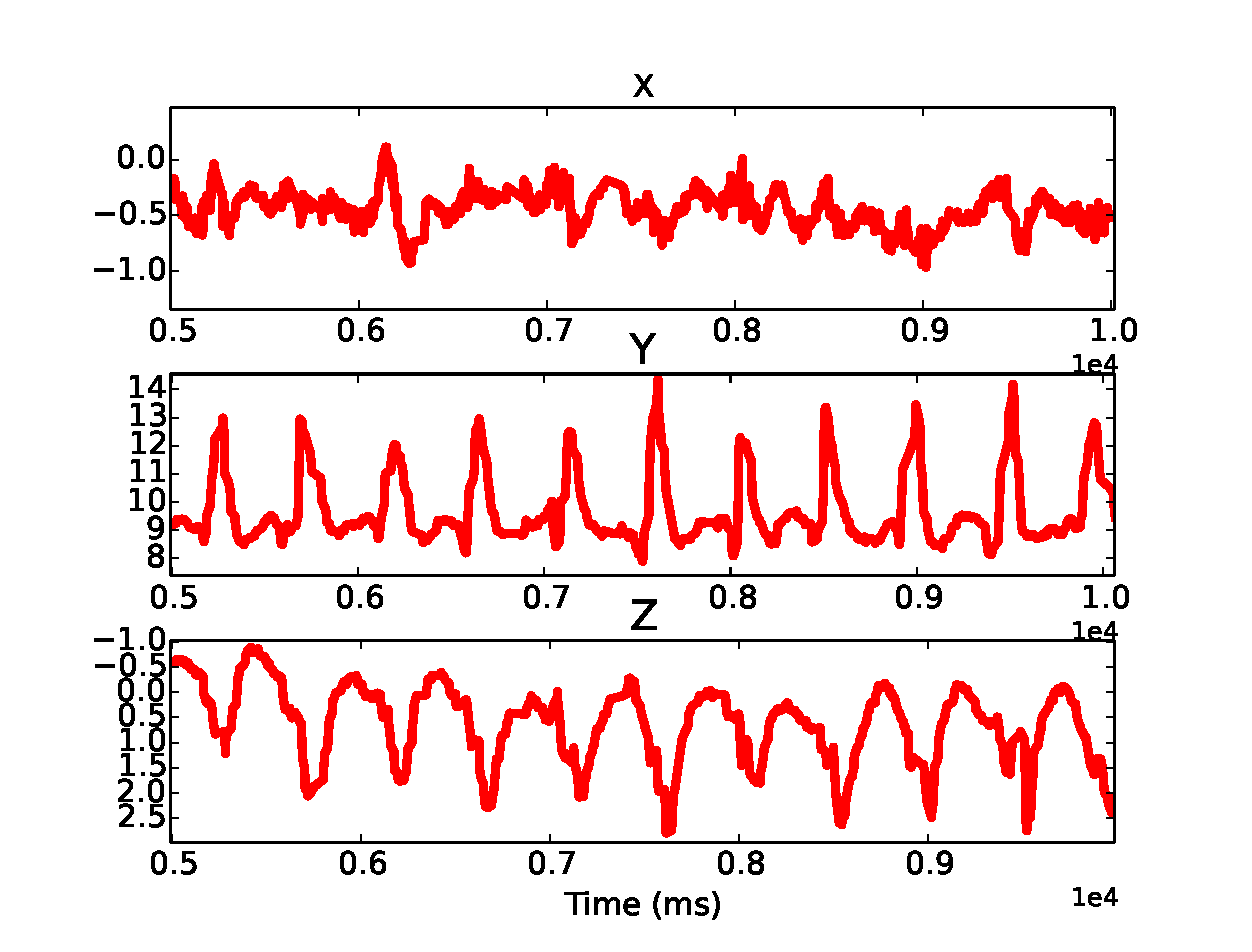
\includegraphics [width=.33\linewidth]{fig/raw_sub1.eps}&
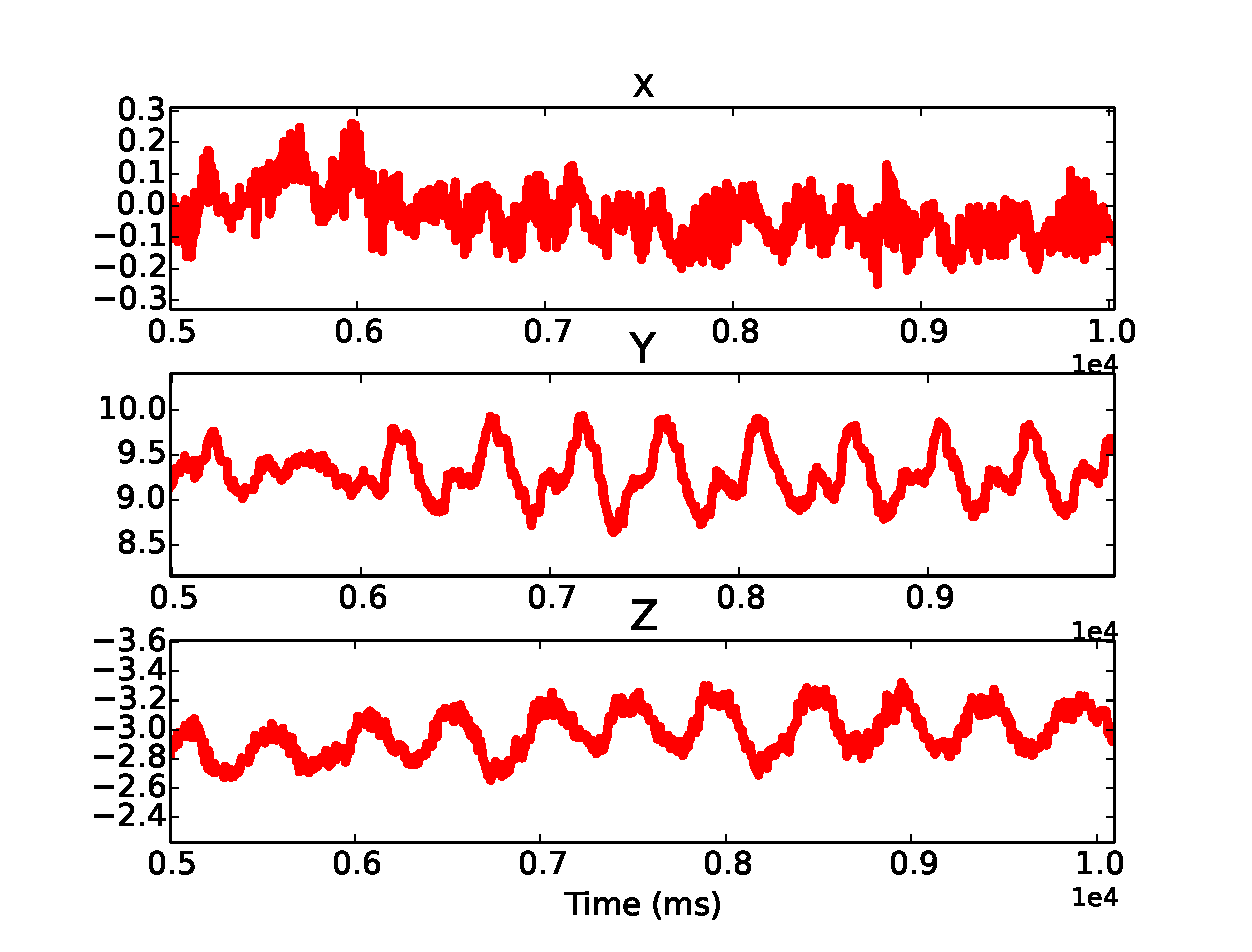
\includegraphics [width=.33\linewidth]{fig/raw_sub8.eps}&
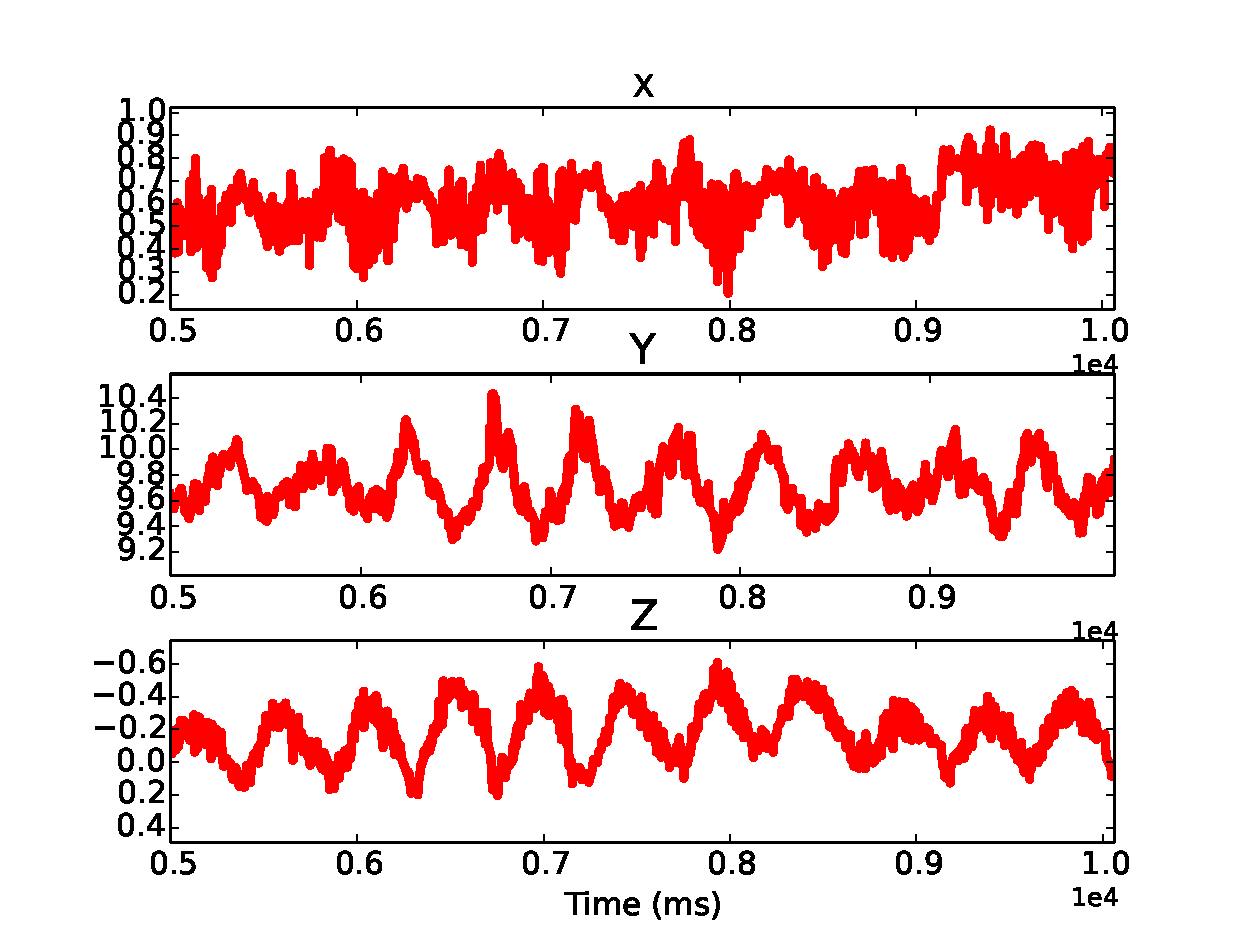
\includegraphics [width=.33\linewidth]{fig/raw_sub3.eps}\\
(a) User 1& (b) User 2 & (c) User 3 \\
\end{tabular}

\begin{tabular}{cc}
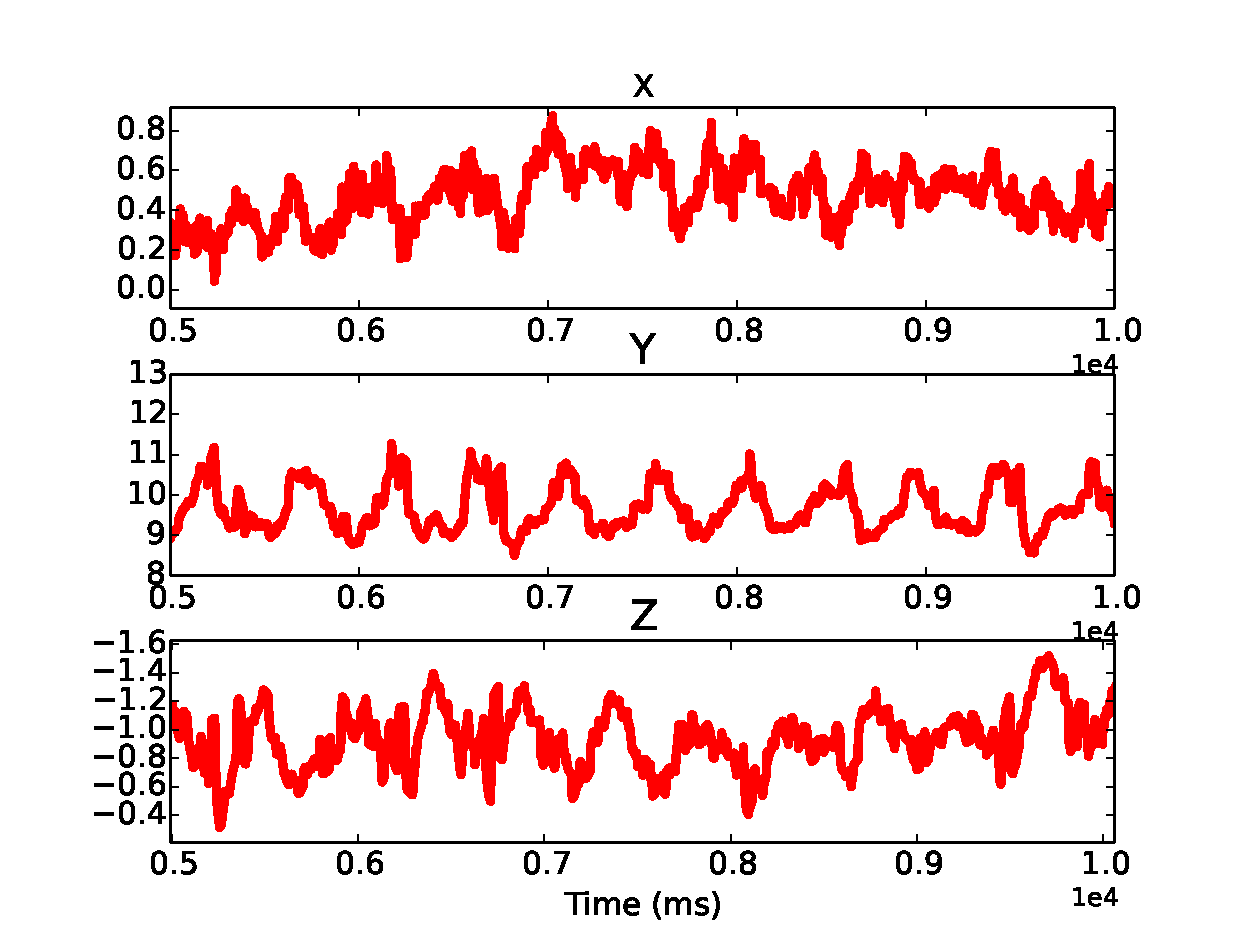
\includegraphics [width=.33\linewidth]{fig/raw_sub4.eps}&
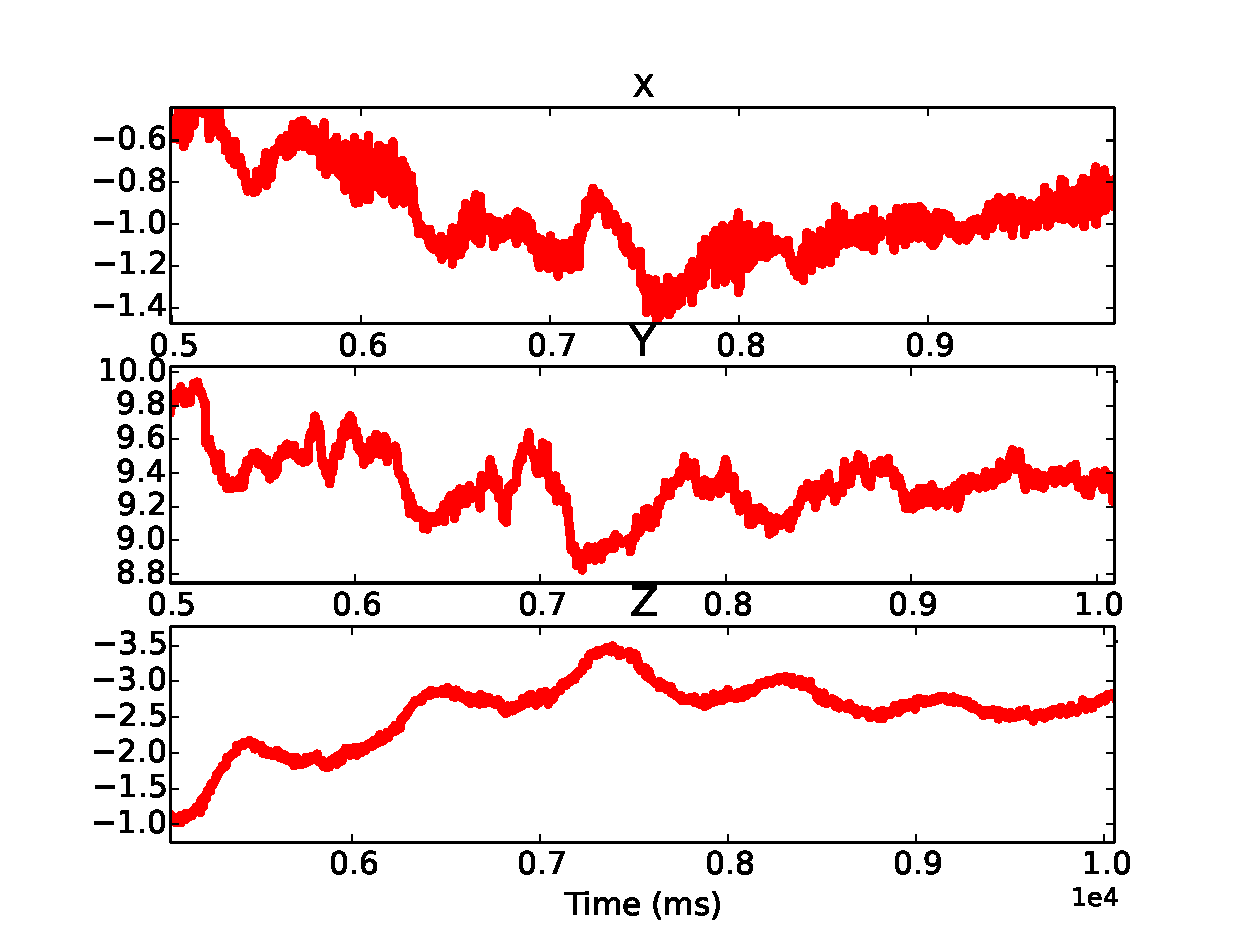
\includegraphics [width=.33\linewidth]{fig/raw_sub5.eps}\\
(d) User 4& (e) User 5 \\
\end{tabular}
\end{center}
\caption{\label{fig:raw} These plots show the raw accelerometer data in the
time domain for five different users when they move their head in response to
a music track wearing the same Google glass. The plots
indicate that different users' head movement patterns appear distinctive from
each other. The five users wore a Google Glass (in turns) and listened to a
10 second audio snapshot of a pop song.}
\end{figure*}

Authentication mechanisms for wearable devices can broadly be divided into two
categories: (i) {\em Direct} authentication, where the users can directly
authenticate themselves to their wearable device using the input/output
interface and/or using signatures generated from the sensors available on the
device, and (ii) {\em Indirect} authentication, where a secondary device --
typically the user's smartphone -- is used as a medium for authentication.
Today's commercially available wearable devices predominantly use the latter
approach where users login to their wearable devices through their smartphone
-- using a PIN or an email account.
%A select few gadgets, for example the Google Glass or fitbit, require the
%users to register their device to their user specific accounts (gmail for
%Google Glass), which can also be perceived as an indirect mechanism for
%authentication.
Unlike the indirect approaches, that require wearable device is registered to
the smartphone and connected (wireless) to the wearable device, direct
mechanisms can leverage from the inbuilt interfaces and sensors on the
wearable device.

%One form of direct authentication is the well-known
%the PIN code approach, however, its effectiveness is only limited to the PIN
%being safe-guarded by the user. A slightly more effective approach would be
%to use a randomly generated code for the user, similar to the RSA
%%keys~\cite{},but that would require a secure and stable wireless connection
%%to the server.
The fact that wearable devices relate significantly to ``what we wear" on the
human body, biometrics can play a key role for direct authentication to
wearable
devices. Biometrics allow a system to identify a user based upon ``who you
are" (i.e., her physiology) instead of ``what you
have'' (i.e., ID cards) or `` what you remember'' (i.e.,
passwords)~\cite{jain2004introduction,o2003comparing,yampolskiy2007motor}.
Physiological biometrics such as DNA, ear shape, face, fingerprint,
hand/finger geometry,
iris, odor, palm-print, retinal scan, and voice, have been very effective and
widely used in many prototype and commercial authentication systems.
In addition, body shape such as body height, width, and body-part proportions
can also be used as biometric cues to identify different
people~\cite{collins2002silhouette}. Even ``soft'' characteristics such as
body weight and fat percentage have been considered as secondary biometrics
for authentication purposes~\cite{ailisto2006soft}. However, biometrics are
not prominently used in wearable devices commercially available today.
While there have been specific point commercial designs (e.g., Nymi~\cite{nymi}), it is unlikely that biometrics will become de-facto standard
for authentication in wearable devices. This can be attributed to the
fact that biometrics would require the specific hardware/sensor available on
the wearable device. Also the overheads for physiological biometrics in
wearable devices can be high, in both, cost for hardware as well as
integration and computing.
%Most of the afore-mentioned biometrics, however, require extra hardware
%(e.g., camera) and/or processing that is too demanding for wearable devices.

An other approach to direct authentication is using behavioral biometrics
where unique signatures from human behavior (subconscious
or in response to external stimulus) provide cues for differentiating and
authenticating users. For example, it has been shown that gait (e.g.,
stride length, the
amount of arm swing) when the user is walking or
running is a reliable identification cue, and irrespective of the
environment~\cite{stevenage1999visual}. Okumura et.al.~\cite{okumura2006study}
have shown that the human arm swing patterns can be used to create signatures
to authenticate to their cell-phones. Monrose
et.al.~\cite{monrose2000keystroke} show that keystroke rhythms, when
users type on the keyboard, that include typing dynamics such as how
long is a keystroke, how far is between consecutive strokes, and how is the
pressure exerted on each key, can be used as a biometric to authenticate
users. Similarly, mouse usage dynamics~\cite{jorgensen2011mouse} and touchpad
touching dynamics~\cite{bo2013silentsense,de2012touch} have also been shown to
serve as potential biometrics.

In comparison to other means of authentication, behavioral biometric
authentication can offer a more convenient (than physiological biometrics),
and more secure (than indirect authentication) solution for wearable device
authentication. With the increasing off-the-shelf
availability and (almost) unlimited access to the sensors on the wearables, it
has become possible to generate and/or infer unique behavioral signatures
specific to users. We use these rationale as a motivation for our proposed
design of a behavioral biometric based authentication that generates unique
signatures from accelerometer signal patterns from user's head movements.
We design an authentication system, dubbed {\em Headbanger}, for head-worn
devices by monitoring user's unique head-movement patterns in response to an
external audio stimulus.

%\vspace{4pt}{\bf Head-movements as a behavioral biometric.}
\subsection{Head-movement as a Biometric}
\label{subsec:headmovements}

%As such, authenticating a user involves comparing her sensor
%readings with the pre-recorded glass owner's sensor readings.
%Our design assumes that there is only one owner per glass, and we can easily
%extend our scheme to handle the cases with multiple owners.
%Figure~\ref{fig:sysarch} presents the system architecture of the \systemname,
%and in the following section, we will discuss each component of this design
%in more detail.

According to~\cite{jain2004introduction}, a human characteristic can be
considered as biometric as long as it is \emph{universal}, \emph{distinctive},
\emph{repeatable}, and \emph{collectible}. With the advancements in head-worn
wearable computer designs it is becoming easier for collecting head-movement
patterns using the inbuilt accelerometers and motion sensors. Such sensors are
available on almost all head-worn wearable devices available today, thus
making head movements that are universally available {\em collectible} in all
aspects. It has been shown~\cite{zentner2010rhythmic} that most people move
their body as a natural response to external rhythmic stimuli such as music --
even at a very early age, infants respond to music and their movements speed
up with the increasing rhythm speed. We observed that even adults naturally
perform head-movements when listening to a fast beat audio track. Based on a
preliminary analysis of the accelerometer signals from five Google Glass
users, we also observed (see Figure~\ref{fig:raw} (a)-(e)) that these users
{\em repeatedly} showed unique and {\em distinctive} head-movement patterns,
when listening to the same music beats on the head-worn device.
Motivated by this observation we hypothesize that head movements
can be a good behavioral biometric characteristic to authenticate
users to their smart glass.
We next formally present the design of our system that
utilizes head-movement patterns as behavioral biometric signature
to authenticate smart glass users.

\iffalse
% moved to next section
\vspace{4pt}{\bf Head-movements as a behavioral biometric.}
%Using a personal imaging device as a running example and through extensive
%experimental evaluation over multiple users we show that our mechanism can
%authenticate users with an acceptance rate greater than 95\% while keeping
%the
%average false rejection rate below 5\%.
%In this study, we propose to establish a smart glass user by capturing her
%unique head movement patterns, and refer to this algorithm as
%\emph{Headbanger}.
According to~\cite{jain2004introduction}, a human characteristic can be
considered as biometric as long as it is \emph{universal}, \emph{distinctive},
\emph{repeatable}, and \emph{collectible}. With the advancements in head-worn
wearable computer designs it is becoming easier for collecting head-movement
patterns using the inbuilt accelerometers and motion sensors. Such sensors are
available on almost all head-worn wearable devices available today, thus
making head-movements that are universally available {\em collectible} in all aspects. It has been
shown~\cite{zentner2010rhythmic} that most people move their body
as a natural response to external rhythmic stimuli such as music -- even at a
very early age, infants respond to music and their movements speed up with the
increasing rhythm speed. We observed that even adults naturally perform
head-movements when listening to a fast beat audio track. Based on a
preliminary analysis of the accelerometer signals from five Google Glass
users\footnote{the five authors wore a Google Glass (in turns) and listened to
a music
beat track for 10 seconds}, we also observed (see Figure~\ref{fig:raw}) that these
users {\em
repeatedly} showed unique and {\em distinctive} head-movement patterns, when
listening to the same music beats while wearing the Glass. As a result, head-movements can be a good behavioral biometric characteristic to authenticate users to their smart glass.

Figures~\ref{fig:raw}(a)-(e) show the raw accelerometer data in the time domain for five different users when they move their head along the same music track wearing the same Google glass. These data demonstrate that different users' head movement patterns are rather distinctive from each other. Motivated by this observation, we next formally investigate how we can utilize head-movement patterns as biometric to authenticate smart glass users.

%** AA: add a figure showing the unique, repeatable and distinctive acc signals
%for head-movements for 5 glass users

% moved to new section
\subsection{Overview of Headbanger}
In this study, we propose to establish a smart glass user by capturing her unique head movement patterns, and refer to this algorithm as \emph{Headbanger}. According to~\cite{jain2004introduction}, a human physiological or behavioral characteristic can be considered as biometric as long as it is \emph{universal}, \emph{distinctive}, \emph{repeatable}, and \emph{collectable}. As far as these four requirements are concerned, it is obvious that head movement is universal and collectable; in this study, we investigate whether it is also distinctive and repeatable. In fact, it has been shown that humans can recognize a person by her overall movement pattern~\cite{loula2005recognizing}, or arm movement pattern~\cite{okumura2006study}. Further, in order to help make a person's head movement easy and repeatable, Headbanger plays fast beat music so that users naturally respond to the music by moving her head in a unique manner.  It has been shown that most people move their body as a natural response to external rhythmic stimuli such as music -- even at a very early age, infants respond to music and move faster when faster rhythm is played~\cite{zentner2010rhythmic}.


\iffalse
Using music-induced head movement as a biometric has several advantages.
First,

%Authentication on commercially available wearable devices today has primarily
%been through the user's
%
%a long list of wearable devices but no standalone authentication method
%
%mostly use two-step authentication - using phone/auxiliary device
%
%gesture based authentication in touch based devices
%
%**AA : how its done in commercial devices. Why is that not sufficient? A
%table
%listing the mechanism for different wearable devices today**

%\subsection{Physiological biometrics}
%Broadly speaking, biometrics can be classified into one of the two
%categories, physiological biometrics and behavioral biometrics. Well-known
%physiological biometrics include DNA, ear shape, face, fingerprint,
%hand/finger geometry, iris, odor, palmprint, retinol scan, and voice, and
%have been used in many prototype and commercial authentication systems.


\fi 